\section{Initial Problem}
\label{sec:initproblem}

In a previous report we documented the work on a system that integrated wearables into a home automation environment in order to provide an interface for controlling devices that are connected to the Internet~\cite{prespecialisation}. 

In the previous report~\cite[pp. 69-73]{prespecialisation} we found that motion gestures can be used to control a home automation environment. We found the system to have an accuracy of 4.29\%, \ie~the correct action was performed 4.29\% of the time. The poor accuracy was due to the use of fine grained position information used when determining which device in the smart home to control.

The position of the user was utilized when determining which device the user points at and thus which device should be controlled. The future work of the report~\cite[pp. 71-73]{prespecialisation} suggests using contextual information to determine which device should be controlled rather than the granular positioning. By doing this it is no longer possible for the user to point at a device in order to control it but we may be able to improve the accuracy of the solution and given the correct contextual information we can narrow the set of devices the user desires to control sufficiently to provide an attractive solution for controlling a smart home.

This report is based on the work done in our previous report.

In the previous report~\cite[pp. 1-4]{prespecialisation} we presented \Cref{fig:wearables-trend,fig:smarthomestrend}. The figures show an increasing trend in wearables and smart homes. Common for wearables and smart homes are that they are both involved in the concept of Internet of Things. As both wearables and smart homes are predicted to be an increasing trend~\cite{WEARABLESTRENDNUMBERS,SMARTHOMETREND}, it is interesting to combine the two in order to make a system that provides an interface for controlling a smart home using a wearable device.

\begin{figure}[!hbt]
  \centering
  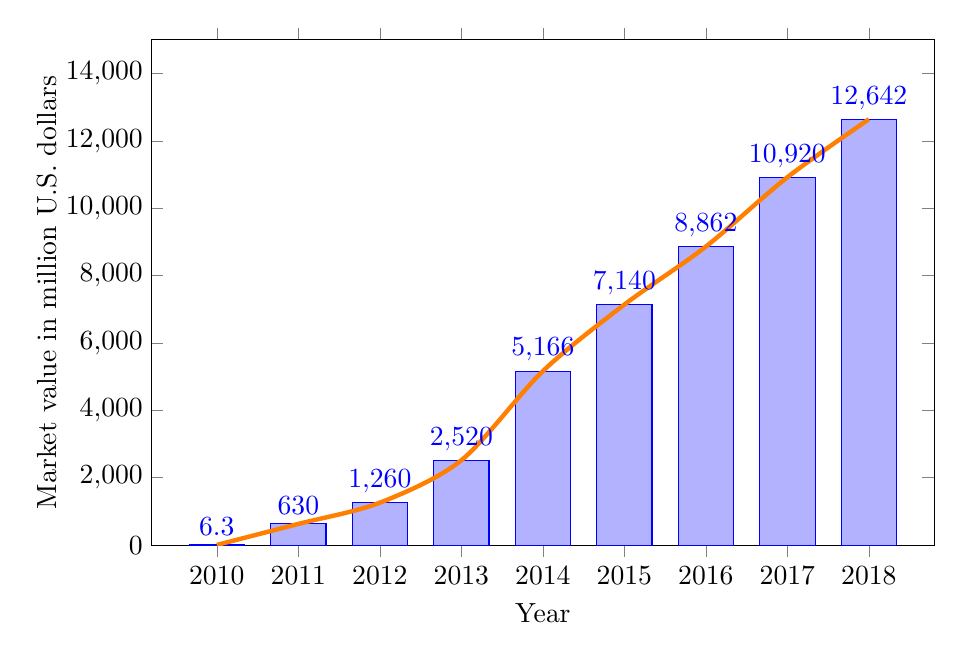
\begin{tikzpicture}
    \begin{axis}[
        height=8cm,
        width=0.95\textwidth,
        xlabel={Year},
        ylabel={Market value in million U.S. dollars},
        yticklabel style={align=right,inner sep=0pt,xshift=-0.3em},
        scaled y ticks = false,
        nodes near coords align={vertical},
        nodes near coords,
        xtick=data,
        symbolic x coords={2010, 2011, 2012, 2013, 2014, 2015, 2016, 2017, 2018},
        ymax=15000,
        ymin=0,
        ybar, 
        bar width=20pt
        ]
        \addplot coordinates {(2010, 6.3) (2011, 630) (2012, 1260) (2013, 2520) (2014, 5166) (2015, 7140) (2016, 8862) (2017, 10920) (2018, 12642)};
        \addplot [ultra thick,orange,line join=round,smooth, nodes near coords = ] coordinates {(2010, 6.3) (2011, 630) (2012, 1260) (2013, 2520) (2014, 5166) (2015, 7140) (2016, 8862) (2017, 10920) (2018, 12642)};
%        
    \end{axis}
\end{tikzpicture}
  \caption{Wearables trend based on sales and statistics. Data from \protect\cite{WEARABLESTRENDNUMBERS}.}
  \label{fig:wearables-trend}
\end{figure}

\begin{figure}[!hbt]
  \centering
  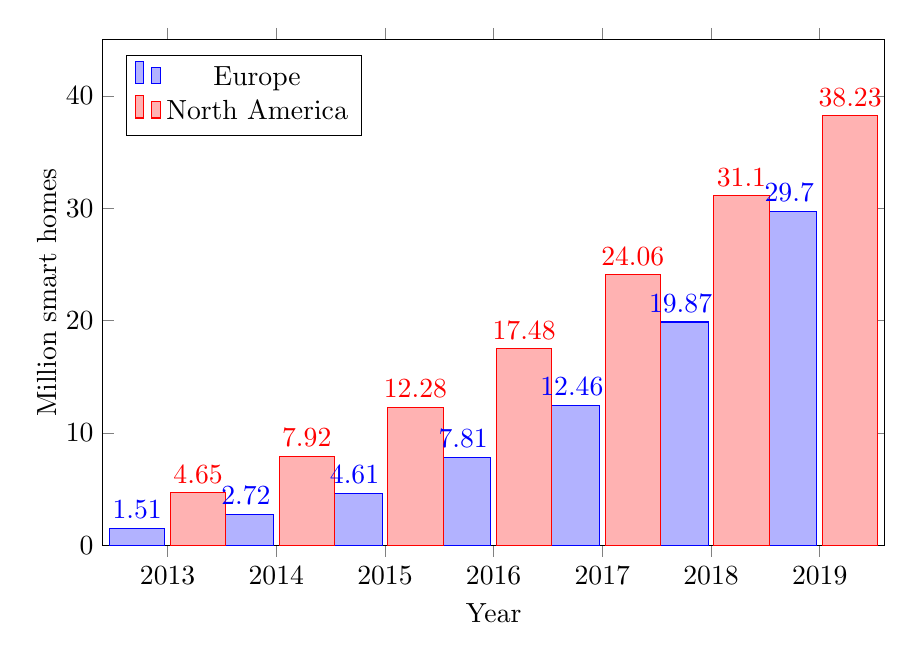
\begin{tikzpicture}
    \begin{axis}[
        height=8cm,
        width=0.95\textwidth,
        xlabel={Year},
        ylabel={Million smart homes},
        yticklabel style={align=right,inner sep=0pt,xshift=-0.3em},
        scaled y ticks = false,
        nodes near coords align={vertical},
        nodes near coords,
        xtick=data,
        symbolic x coords={2013, 2014, 2015, 2016, 2017, 2018, 2019},
        ybar,
        ymax=45,
        ymin=0,
        bar width=20pt,
        legend pos = north west,
        ]
        \addplot coordinates {(2013, 1.51) (2014, 2.72) (2015, 4.61) (2016, 7.81) (2017, 12.46) (2018, 19.87) (2019, 29.70)};        
        \addplot coordinates {(2013, 4.65) (2014, 7.92) (2015, 12.28) (2016, 17.48) (2017, 24.06) (2018, 31.10) (2019, 38.23)};
        \legend{Europe, North America}
        
        %Trend lines:
%        \addplot [ultra thick,orange,line join=round,smooth, nodes near coords = ] coordinates {(2013, 1.51) (2014, 2.72) (2015, 4.61) (2016, 7.81) (2017, 12.46) (2018, 19.87) (2019, 29.70)};
%        \addplot [ultra thick,orange,line join=round,smooth, nodes near coords = ] coordinates {(2013, 4.65) (2014, 7.92) (2015, 12.28) (2016, 17.48) (2017, 24.06) (2018, 31.10) (2019, 38.23)};
%        

    \end{axis}
\end{tikzpicture}
  \caption{Smart homes trend based on sales and statistics. Data from \protect\cite{SMARTHOMETREND}.}
  \label{fig:smarthomestrend}
\end{figure}

The definition of a \emph{smart home system} is  that the system uses a smartphone application or a web portal as a user interface~\cite{SMARTHOMETREND}. Therefore the numbers presented in \Cref{fig:smarthomestrend} does not include homes controlled solely by switches, timers, sensors and remote controls.

In order for a web portal or a smartphone application to provide meaningful functionality in a smart home system, the software should provide some mechanism for controlling or monitoring devices in the home. In order to do this, the devices are accessible using some technology for exchanging data, \eg~WiFi or Bluetooth. These devices are involved in the concept of Internet of Things. 

While not directly related to the concept of a smart home, a wearable device can play a role in a smart home. The wearable device can provide the application used for interacting with devices in the smart home.

Note that the definition of a smart home system as presented in~\cite{SMARTHOMETREND} does not include to which degree the smartphone application or web portal is involved in the system. A simple system including a smartphone application with a single button for turning a light on and off is a \emph{smart home system}.

We accept the definition of a smart home presented in~\cite{SMARTHOMETREND} and formulate it as shown in \Cref{def:smarthome} as it is sufficient for our use in that we are interested in replacing the smartphone application with an application running on wearable device.

\begin{definition}
\label{def:smarthome}
A smart home, is a home that can be controlled using a smartphone application or a web porta as a user interface.
\end{definition}

%%% Local Variables:
%%% mode: latex
%%% TeX-master: "../../master"
%%% End:
